\chapter{Cell type classification of sparse single-cell RNA-seq data} \label{chap:3}

\section{Background}

Recent advances in scRNA-seq are enabling higher numbers of cells to be sequenced than ever before. Specifically, droplet-based scRNA-seq protocols are now enabling the sequencing of tens of thousands of cells at a time, thereby enabling the study of cell populations at unprecedented scales and levels of granularity (\citealp{TabulaMuris2018, Zheng2017, Macosko2015}).  Unfortunately, the ability to sequence high volumes of cells comes at the cost of capturing fewer reads per cell, leading to fewer measured genes per cell (Fig.~\ref{fig:sparsity}).  This data sparsity introduces challenges to cell type classification because there is less data to inform each cell's cell type.  

 \begin{figure}[h!]
      \centerline{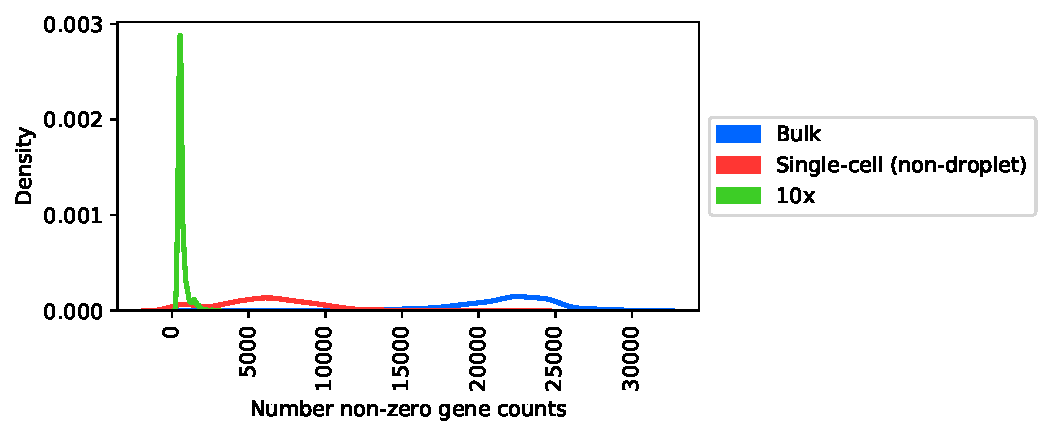
\includegraphics[width=13cm]{figures/num_genes_expressed_distribution.pdf}}
      \caption{\textbf{Sparsity of single-cell assays.} Comparing the sparsity between the bulk RNA-seq dataset, the non-droplet-based scRNA-seq dataset from Chapter~\ref{chap:2}, and 5,000 random cells from the \cite{Zhang2018} 10x scRNA-seq dataset described in Section~\ref{sec:sparse_data}.}
      \label{fig:sparsity}
      \end{figure} 

As these scRNA-seq datasets grow ever larger, rapid cell type classifiers will become more necessary.  This is especially true if this technology is to ever be deployed in a clinical setting where time and computational resources are limited.  The vision is that scRNA-seq will enable new diagnostic tests that entail measuring the transcriptome of specific cell populations (\citealp{Haque2017}).  Due to the limit on computational resources in the clinic, such applications may require phenotyping of individual cells in a streaming fashion where phenotyping is performed on one cell at a time independently from the rest of the cells.  As in Chapter~\ref{chap:2}, we focus on the cell type classification task; however, the methodologies pursued in this chapter may carryover to other single-cell phenotyping tasks. 

The most common techniques for classifying cell type using bulk RNA-seq datasets take a reference-based (i.e. nearest-neighbors-based) classification approach by matching each cell to the most similar bulk RNA-seq expression profile in the reference set (i.e. training set).  Two such methods that take this approach are scMatch (\citealp{Hou2019}) and singleR (\citealp{Aran2019}).  Unfortunately, reference-based classification is computationally expensive with large memory requirements for storing the reference data.  

Very recent work has proposed using neural networks to perform cell type classification on human data (\citealp{Xie2019, Ma2019}). Such an approach may also enable rapid cell type classification as these models do not require extensive computation at test-tme. We note, however, that these methods train on scRNA-seq data, rather than bulk. We also note that neural networks do not easily enable taking into account the hierarchy of cell types, whereas the methods developed in this chapter simply extend binary cell type classifiers and therefore can be easily inserted in to the ensemble-based hierarchical classification frameworks discussed in Chapter~\ref{chap:2}.  

The models developed in Chapter~\ref{chap:2} promise an avenue for efficient and accurate cell type classification. Unfortunately, the models developed in Chapter~\ref{chap:2} were trained on dense, bulk RNA-seq data and therefore, out of the box, they may not be optimal for use on sparse scRNA-seq data.  This chapter addresses this issue by exploring methods for adapting these bulk-trained classifiers for use on sparse scRNA-seq data. To this end, we explored two general strategies for transforming the test data, making it more dense so that it better resembles the training data.  

To this end, we explored two general strategies for adapting the bulk-trained classifiers to sparse data: in the first strategy, we transform the bulk RNA-seq test data, making it more sparse, so that its sparsity matches that of the test data. In the second strategy, we transform the test data, making it more dense so that it better resembles the training data.  

%First, these models have relatively small storage requirements as they need only store the per-gene coefficients for each cell type ($L \times G$ coefficients where $L$ is the number of cell type labels and $G$ is the number of genes), rather than the full reference dataset ($N \times G$ values where $N$ is the number of samples in the reference set). Second, these models allow for fast prediction time as each cell type is associated with a linear model.  Therefore running a query dataset through these models requires a single matrix multiplication step followed by the hierarchical correction step (e.g. isotonic regression).  


Next, we explore the use of gene expression imputation algorithms. Gene expression imputation on scRNA-seq is the task of imputing counts for genes. Emerging approaches for gene expression imputation entail pooling data across cells in the query dataset (\citealp{Dijk2018, Huang2018, Li2018}).  Because these approaches pool data across the query dataset, they require computing on the entire dataset at once and therefore are not apt for a setting in which phenotyping must either be parallelized across cells or in which phenotyping must be performed in a streaming fashion. To address this shortcoming, we develop a novel probabilistic model of the sparse scRNA-seq data-generating process, which implicitly performs gene expression imputation and allows for most computation to occur on the training set, thereby enabling rapid cell type classification in a streaming fashion. 
 
\section{Data}\label{sec:sparse_data}

For the experiments used in this chapter, we utilized both data from Chapter~\ref{chap:2} as well as 10x scRNA-seq data from  \cite{Zhang2018}. We used the bulk RNA-seq data from Chapter~\ref{chap:2} to simulate scRNA-seq data. Specifically, for a given number of total reads $n$ (i.e. level of sparsity), for each sample, we sampled a sparse expression profile according to a multinomial distribution:
 $$\bold{x}_{\text{sparse}} \sim \text{Mult}(n, p_1, \dots, p_G)$$
 where $G$ is the total number of genes and $p_i$ is the fraction of reads assigned to gene $i$.  We created four sparsified versions of the dataset corresponding to four values for $n$: $10^5$, $10^4$, $10^3$, and 100 reads. 
 
 As a test set, we used Chromium 10x scRNA-seq data from \cite{Zhang2018}. Specifically, we used ten peripheral blood mononuclear cell (PBMC) datasets, where each consists of a purified, immune cell type\\(\texttt{https://support.10xgenomics.com/single-cell-gene-expression/datasets}). This dataset is summarized in Table~\ref{tab:10x_pbmc}.  We note that this 10x dataset provides counts for \NumTenXGenes{} genes rather than \GeneLevelFeatures{} genes used in the dataset from Chapter~\ref{chap:2}.  The intersection of these two gene sets was \NumTenXIntersection{} total genes.  We therefore only used these  \NumTenXIntersection{} so that we could train classifiers on our dataset and apply them directly to this 10x data.
 
 \begin{table}[h!]
    \begin{center}
    \begin{tabular}{ |l|c| } 
    \hline
    \textbf{Cell type} & \textbf{No. of cells} \\ \hline
    CD8+/CD45RA+ Naive Cytotoxic T Cells & 11,953  \\
    CD4+ Helper T Cells & 11,213 \\
    CD4+/CD45RA+/CD25- Naive T cells & 10,479  \\
    CD4+/CD25+ Regulatory T Cells & 10,263  \\
    CD4+/CD45RO+ Memory T Cells & 10,224 \\
    CD8+ Cytotoxic T cells & 10,209  \\
    CD19+ B Cells & 10,085  \\
    CD34+ Cells & 9,232  \\
    CD56+ Natural Killer Cells & 8,385 \\    
    CD14+ Monocytes & 2,612 \\
     \hline
    \end{tabular}
    \end{center}
    \caption{\textbf{10x Dataset Summary.} A summary of the ten PBMC FAC-sorted cell types from \cite{Zhang2018}.}
    \label{tab:10x_pbmc}
    \end{table}


 
\section{Results and Discussion}

\subsection{Performance degradation on sparse data}\label{sec:sparse_test}
 
 We first performed an experiment to assess how well the trained classifiers from Chapter~\ref{chap:2} perform on sparse RNA-seq data out-of-the-box.  In this experiment, we applied the independent one-versus-rest classifiers trained on the bulk RNA-seq training set to each of the sparse versions of the test set described in Section~\ref{sec:sparse_data}.  As expected, we found a strong decrease in performance as sparsity increased (Fig.~\ref{fig:results_test_bulk_downsample}).  

 \begin{figure}[h!]
      \centerline{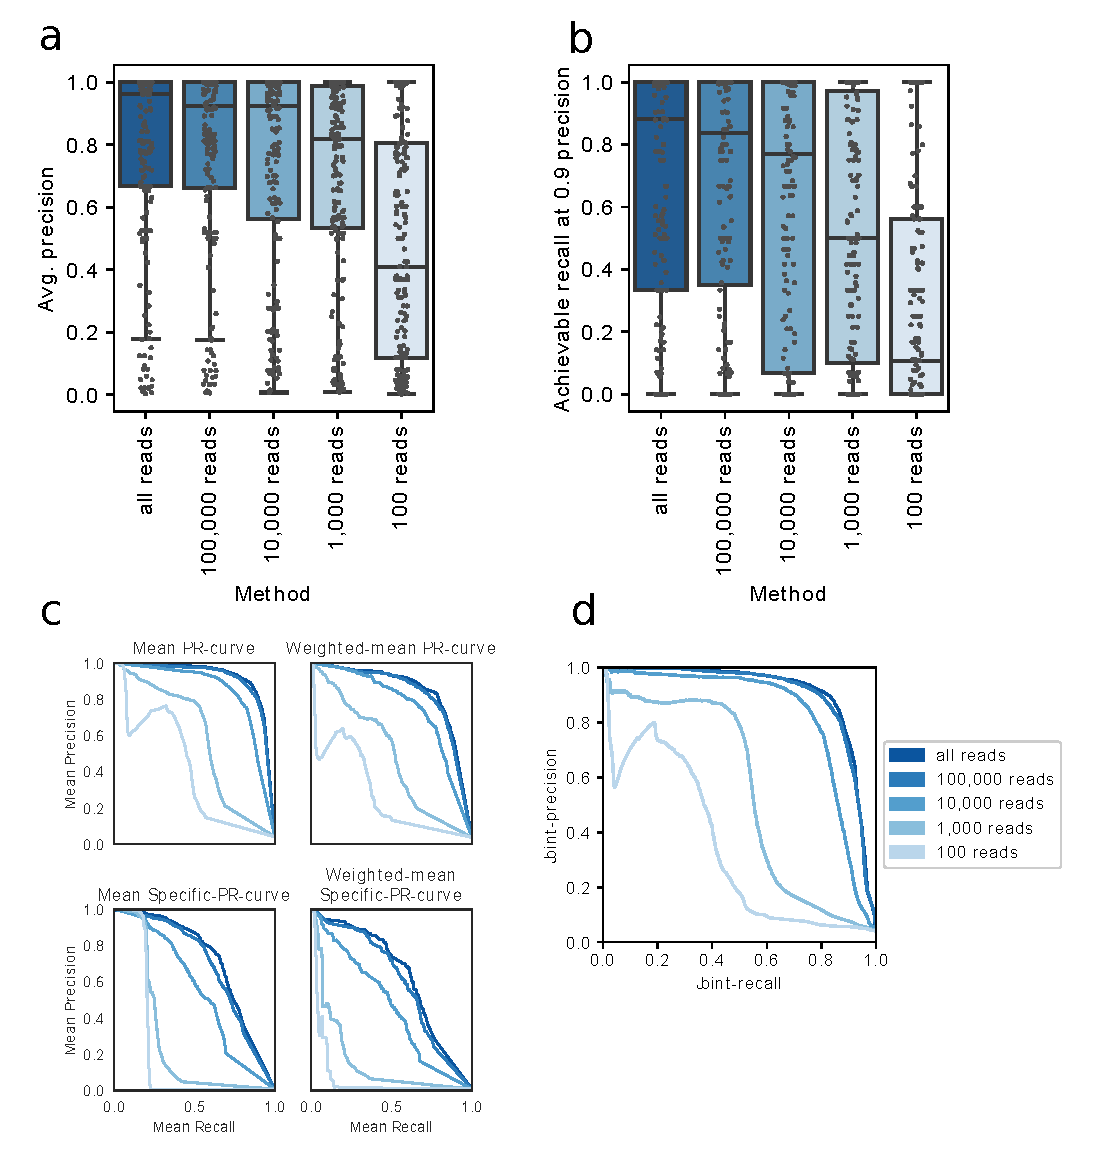
\includegraphics[width=13cm]{figures/bulk_test_set_downsampled_results.pdf}}
      \caption{\textbf{Results on sparse test set.} (a) Comparison between the distributions of average-precision generated by each method across all cell types.  (b) Comparison of the distributions over the highest achievable recalls when precision is fixed at 0.9 across all cell types. (c) Variants of the mean precision-recall curves for comparing the average performance of each method across all samples. (d) The joint-precision recall curves for all methods generated by ranking all sample-cell type output probabilities jointly.}
      \label{fig:results_test_bulk_downsample}
      \end{figure}

\subsection{Training on sparsified bulk RNA-seq data}\label{sec:sparse_test}

We explored an approach in which we trained the classifiers on sparsified bulk RNA-seq data in order to test whether matching the sparseness of the training data to the test data would improve performance. We first  compared the performance of the classifier trained and tested at each level of sparsity to that trained on the full, dense data (Fig.~\ref{fig:results_train_and_test_bulk_downsample}). As expected, we see that training on data that matches the sparsity of the test data improved performance at all read-depths across all modes of evaluation.


%We found that at higher read-depths, training on sparse data tended to hurt performance. Only at very low read-depths did we see a gain in performance when training on data whose sparsity matched the sparsity of the test data.  Interestingly, in the joint evaluation, we found that lower levels of sparsity yielded much poorer performance. Notably, the classifiers that were trained and tested on data sampled down to $10^5$ reads produced the poorest joint PR-curve (Fig.~\ref{fig:results_train_and_test_bulk_downsample}c), even worse than the classifiers trained and tested on data sampled down to 100 reads.  Examining the errors by these classifiers revealed that the independent cell type classifiers were poorly calibrated as indicated by the germ cell classifiers incorrectly producing very high probabilities for most of the test samples (thus, causing the highly ranked predictions to be incorrect when computing the joint PR-curve).  	

 \begin{figure}[h!]
      \centerline{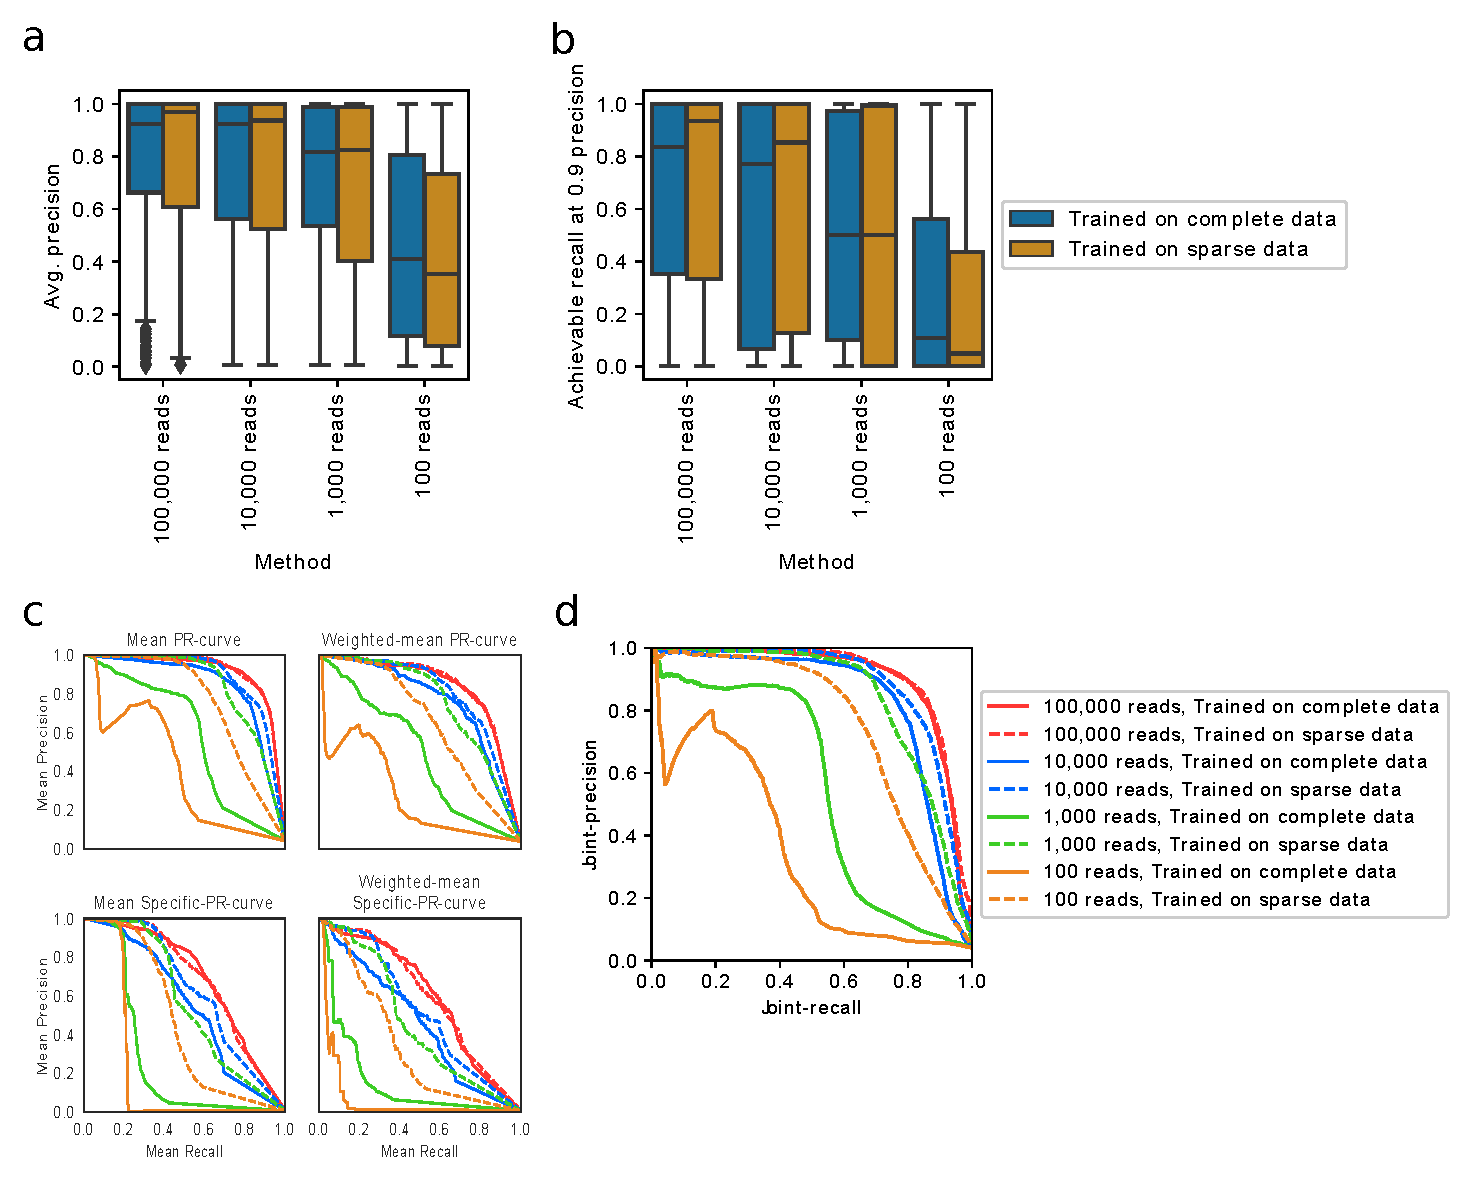
\includegraphics[width=13cm]{figures/bulk_train_and_test_downsampled_results.pdf}}
      \caption{\textbf{Results training on sparse training data and testing on sparse test set.} (a) Comparison between the distributions of average-precision generated by each method across all cell types.  (b) Comparison of the distributions over the highest chievable recalls when precision is fixed at 0.9 across all cell types. (c) Variants of the mean precision-recall curves for comparing the average performance of each method across all samples. (d) The joint-precision recall curves for all methods generated by ranking all sample-cell type output probabilities jointly.}
      \label{fig:results_train_and_test_bulk_downsample}
      \end{figure}

Next, we trained a classifier on a version of the complete bulk RNA-seq dataset (i.e. the union of the training and test sets) that was downsampled to 25,000 reads, which was the approximate number of reads in each 10x sample. We then applied the classifier trained on this downsampled data to the 10x data. As before, we found this classifier to outperform the classifier that was trained on the full, non-downsampled bulk RNA-seq training set (Fig.~\ref{fig:10x_results}).

\subsection{Testing on imputed, sparse scRNA-seq data}

Unfortunately, in order to improve the classifiers by training on sparse data, the sparsity of the training data should match the test data. This cannot be assumed as differing scRNA-seq datasets will often have differing read-depths. Therefore, we also explored an approach in which we train the classifiers on the full, bulk RNA-seq data and then apply them to sparse scRNA-seq data that has undergone gene expression imputation.  Because gene expression imputation requires pooling data across cells in a large collection of scRNA-seq data, this approach was not apt for application to the sparsified bulk RNA-seq dataset. Therefore, we only tested these methods on the 10x dataset.  Specifically, we trained one-vs.-rest cell type classifiers on the full set of bulk RNA-seq data using only the \NumTenXIntersection{} that also were present in the 10x dataset. Before testing these models on the 10x data, we imputed the expression of genes using MAGIC (\citealp{Dijk2018}), which uses a graph diffusion procedure on the single-cell nearest-neighbors graph.  We ran MAGIC in two modes of operation: an "optimistic mode" and a "realistic mode".  In the "optimistic" mode of operation, we ran MAGIC on each 10x PBMC cell type separately (i.e. we ran MAGIC separately on the data represented by each row of Table~\ref{tab:10x_pbmc}).  In this mode, only cells of the same cell type share information during the imputation process, thereby mitigating the possibility that the algorithm will incorrectly use cells of one cell type to impute the missing gene values within a cell of a differing cell type.  This mode of operation therefore provides results that serve as a sort of upper bound on the potential of gene expression imputation.  In the "realistic" mode of evaluation, we ran MAGIC on the entire PBMC dataset jointly, which better resembles how this tool is used in practice (i.e. the query data usually consists of heterogeneous cell types and information is potentially shared across cells from differing cell types).

Perhaps unsurprisingly, running MAGIC in the "optimistic" mode resulted in very high performance, which indicates that collectively, the cells contain the information for performing accurate classification, but that sparsity within a given cell makes classification difficult.  We also found that performing MAGIC in the "realistic" mode led to improvement over the application of the classifiers on the non-imputed data. 

 \begin{figure}[h!]
      \centerline{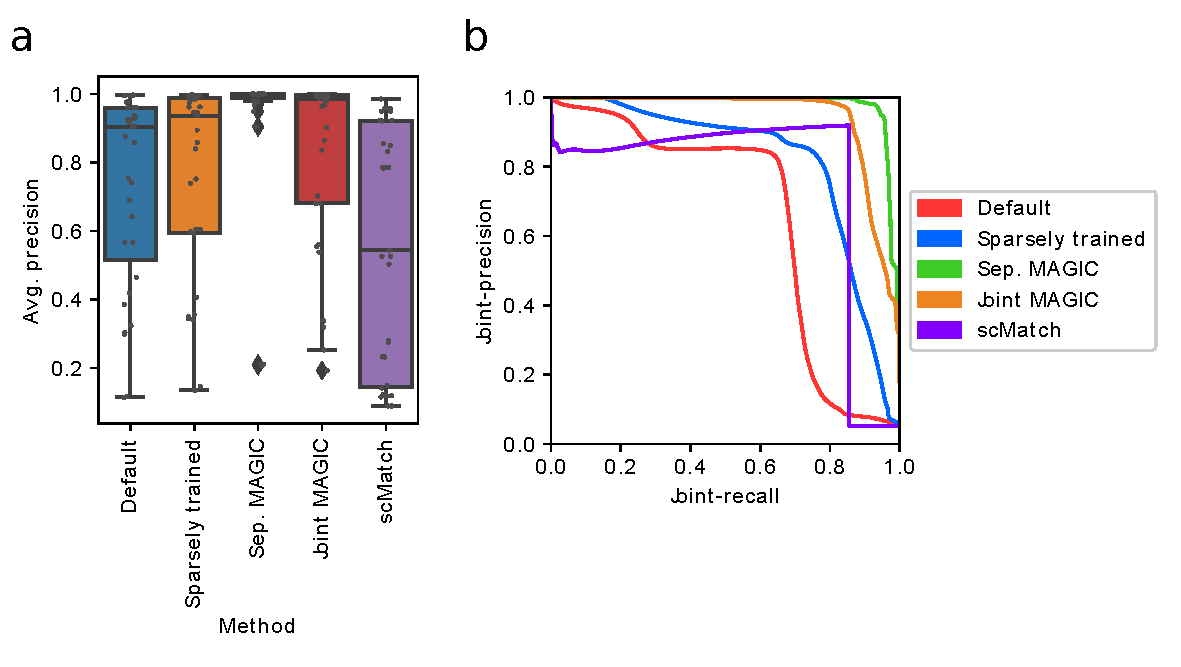
\includegraphics[width=13cm]{figures/10x_results.pdf}}
      \caption{\textbf{Results on 10x dataset.} (a) Comparison between the distributions of average-precision generated by each method across all cell types.  (b) Comparison of the distributions over the highest achievable recalls when precision is fixed at 0.9 across all cell types.}
      \label{fig:10x_results}
      \end{figure}

 \begin{figure}[h!]
      \centerline{\includegraphics[width=18cm]{figures/10x_pr_curves_on_graph.pdf}}
      \caption{\textbf{10x test set precision-recall curves.} Precision-recall curves for each cell type on the 10x scRNA-seq test dataset. Each node is colored according to which method yielded the highest average precision (red = default classifiers, blue = sparsely trained classifiers, green = running MAGIC on each separate cell type, orange = running MAGIC on the entire 10x dataset, purple = scMatch). The intensity of the color corresponds to the difference between the highest average-precision and the second highest average-precision achieved for that node.}
      \label{fig:10x_pr_curves}
      \end{figure}



\subsection{Baseline reference-based approach}

In reference-based classification, each cell's expression profile is queried against a set of bulk reference expression profiles. The cell is then assigned the cell type pertaining to the most similar sample in the reference set.  As a representative example of a reference-based classifier, we used a recent method called scMatch  (\citealp{Hou2019}). We ran scMatch with the default settings, which uses the FANTOM5 database (\citealp{Lizio2017}) as a reference set and uses Spearman correlation as the similarity metric.   We found the independent one-vs.-rest models trained in Chapter~\ref{chap:2} outperfomed scMatch in the per cell type mode of evaluation (Fig.~\ref{fig:10x_results}), but underperformed scMatch in the joint-evaluation. This indicates that scMatch tended to yield more accurate classifications on more general, and therefore more common, cell types (Fig.~\ref{fig:10x_pr_curves}). When preprocessing the test data with MAGIC, our classifiers outperformed scMatch on both the per cell type and joint modes of evaluation (Fig.~\ref{fig:10x_results}, Fig.~\ref{fig:10x_pr_curves}).


\subsection{A probabilistic generative model for cell type classification of sparse data}\label{sec:sc_new_model}

Because gene expression imputation algorithms must compute on the entire query set, these algorithms cannot be deployed in a situation that requires either parallelizing classification across cells or performing cell type classification in a streaming fashion where cell type classification is performed on one cell at a time independently from the rest of the cells.   To address this shortcoming, we propose a novel method for adapting the bulk RNA-seq-trained classifiers from Chapter~\ref{chap:2} that is based on a probabilistic model of the sparse scRNA-seq data-generating process.  In this model we treat the sparse RNA-seq expression profile as an observed random variable and posit that this sparse expression profile was ``generated" from an unobserved, dense RNA-seq expression profile.  In order to perform binary classification for a given cell type, we compute the marginal probability that the sample is of the given cell type conditioned on the sparse data.  We hypothesize that if we can accurately model the latent random variable representing the dense expression profile so that it resembles the bulk RNA-seq data on which the classifier was trained, then our classifier will more accurately predict the sample's cell type.  


\subsubsection{Model description}

To more rigorously describe the model, we will introduce some notation. Let $\bold{x} \in \mathbb{N}^G$ be the observed sparse RNA-seq expression profile, where $G$ is the number of genes, and $x_i$ is the read count for gene $i$.  Let $s := \sum_{i=1}^G x_i \times 10^{-6}$ be the scaled read-depth for the observed scRNA-seq sample. Let $\bold{y} \in \{0, 1\}^L$ be the cell type assignments for $L$ cell types. That is $y_i \in \{0, 1\}$ indicates whether the cell belongs to cell type $i$.  We let $\bold{z} \in \mathbb{R}^G$ be a latent, dense expression profile, in units of counts per million (CPM), from which $\bold{x}$ was generated.  Further, we assume that $\bold{z}$ was sampled from one of $K$ gamma distributions\footnote{As shorthand, for a multivariate random variable $\bold{X} \in \mathbb{R}^n$, $\bold{X} \sim \text{Gamma}(\bold{a}, \bold{b})$ denotes the joint distribution of $\bold{X}$ where each element $X_i$ is independent of the rest and distributed according to $X_i \sim \text{Gamma}(a_i, b_i)$. Similarly, $\bold{X} \sim \text{Poisson}(\boldsymbol{\lambda})$ denotes that the elements are independent and distributed according to $X_i \sim \text{Poisson}(\lambda_i)$}, indicated by the random variable $k \in [K]$. We let $\bold{A} \in \mathbb{R}_{+}^{K \times G}$ be the matrix of shape parameters and $\bold{B} \in \mathbb{R}_{+}^{K \times G}$  be the matrix of rate parameters for these $K$ mixture components where $\bold{a}_k$ and $\bold{b}_k$ are the shape and rate parameters respectively of the $k$th component. We let $\boldsymbol{\phi} \in [0,1]^K$, where $\sum_{i=1}^K \phi_i = 1$, be the prior probabilities of drawing a sample from each mixture component.  We use $\sigma(x)$ to denote the logistic function:
$$\sigma(x) := \left[1 + \exp(-x)\right]^{-1}$$
Then, the full data-generating process (Fig.~\ref{fig:sc_graphical_model}) is as follows:
\begin{enumerate}
\item $k \sim \text{Categorical}(\boldsymbol{\phi})$
%\item For each gene $i \in [G]$:
\item $\bold{z} \sim \text{Gamma}(\bold{a}_k, \bold{b}_k)$
\item $\bold{x} \sim \text{Poisson}\left(\bold{z}s\right)$
\item For each cell type $i \in [L]$:
\begin{itemize}
\item $y_i \sim \text{Bernoulli}\left(\sigma\left(\boldsymbol{\beta}_i^T \log(\bold{z}+1)\right)\right)$
\end{itemize}
\end{enumerate}
To make a prediction for cell type $i \in [L]$, we compute the marginal probability of the cell type assignment $y_i$ conditioned on the observed, sparse data $\bold{x}$:
\begin{align*}
p(y_i=1 \mid \bold{x}) &= \sum_{k=1}^K \int_{\bold{z}} p\left(y=1 \mid \bold{z}\right) p\left(\bold{z} \mid \bold{x}, k\right) p\left(k \mid \bold{x}\right) \ d\bold{z} \\
&= \sum_{k=1}^K p(k \mid \bold{x}) E_{\bold{z} \mid \bold{x}, k} \left[p\left(y=1 \mid \bold{z}\right)\right]
\end{align*}
where 
$$p\left(y=1 \mid \bold{z}\right) = \sigma\left(\boldsymbol{\beta}_i^T\log(\bold{z}+1)\right)$$
and
$$\bold{z} \mid \bold{x}, k \sim \text{Gamma}(\bold{x}+\bold{a}_k, \bold{b}_k + s)$$
and 
$$p(k \mid \bold{x}) = \frac{ \phi_k \prod_{i=1}^G f_{\text{NegBin}}\left(x_i ; a_{k,i}, \frac{s}{s + b_{k,i}} \right)}{\sum_{k'=1}^K \phi_{k'} \prod_{i=1}^G f_{\text{NegBin}}\left(x_i ; a_{k',i}, \frac{s}{s + b_{k',i}} \right)}$$
where
$$f_{\text{NegBin}}(x; r, p) := \frac{\Gamma(x + r)}{x! \Gamma(r)} p^x(1-p)^r$$ 
is the probability density function for the Negative Binomial distribution, and
$$\Gamma(x) := \int_{0}^{\infty} z^{x-1}e^{-z} dz,$$
is the gamma function  (See Appendix~\ref{app:model_deriv} for full derivation of these probabilities).  

 \begin{figure}[h!]
      \centerline{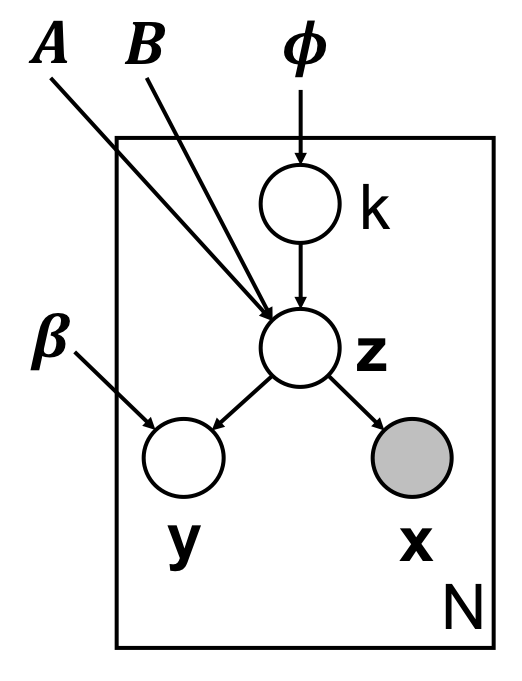
\includegraphics[scale=0.65]{figures/sc_graphical_model.png}}
      \caption{\textbf{Graphical model for sparse cell type classification.} The probabilistic graphical model for performing cell type classification on sparse RNA-seq data represented in plate notation.}
      \label{fig:sc_graphical_model}
      \end{figure}

\subsubsection{Model training and inference}

This model requires the specification of the gamma-mixture distribution over the latent, dense expression profile $\bold{z}$.  Specifically, we must specify the gamma shape and rate parameters, $\bold{A} \in \mathbb{R}^{G \times K}$ and $\bold{B} \in \mathbb{R}^{G \times K}$ respectively, for all K clusters.  As a first approach to specifying this distribution, we propose a two-step process that entails first clustering the bulk RNA-seq training data and then using each cluster to estimate a joint distribution over the CPM values for each gene where each gene is independent and gamma-distributed.    This process introduces a number of modeling choices in regards to which clustering algorithm to deploy as well as how each gamma distribution is to be estimated.

When applying the trained model to query data, one must compute $p(y_i=1 \mid \bold{x})$, which requires the calculation of an expectation. Unfortunately, this expectation does not admit a ready closed-form solution.  Instead, it must be approximated either through Monte Carlo integration\footnote{Monte Carlo integration of an expectation $E(f(X))$ involves sampling $n$ samples $x_1,\dots,x_n \overset{\text{i.i.d.}}{\sim} X$ and then approximating the expectation via $\frac{1}{n}\sum_{i=1}^n f(x_i)$. } or through an analytical approximation.  For the remainder of this chapter, we deployed Monte Carlo integration, finding that the variance of the expectation was low with 100 samples.  Future work will entail developing an accurate analytical approximation.

\subsubsection{Relationship to existing approaches}

We note that the model presented in this chapter has similarities to recent bulk RNA-seq-informed gene expression imputation algorithms.  Specifically, SCRABBLE (\citealp{Peng2019}) and URSM (\citealp{Zhu2018}) were developed to utilize a bulk RNA-seq dataset to inform the value of missing genes in the target scRNA-seq data.  SCRABBLE sets up an optimization problem in which the goal is to find a dense representation of the scRNA-seq dataset for which the aggregate of the imputed expression profiles most closely resembles the bulk RNA-seq data.  In contrast, URSM is more related to the model proposed in this chapter in that URSM also proposes a joint probabilistic model over both the scRNA-seq data as well as the bulk RNA-seq data.  Importantly both SCRABBLE and URSM assume that that the bulk RNA-seq sample provided as input to the imputation algorithm represents a mixture of the cell types present in the target scRNA-seq dataset. Therefore, these methods are most apt for scenarios in which a bulk RNA-seq sample can be obtained from the same biological sample as that from which the scRNA-seq sample was obtained.  In this chapter, this assumption cannot be made as we seek to leverage the trove of heterogenous, publicly available bulk RNA-seq data.

We also point out similarities between this model and the SAVER algorithm for gene expression imputation (\citealp{Huang2018}). To perform imputation, SAVER assumes a similar gamma-poisson generative process of the scRNA-seq data where each cell is generated by first sampling a rate parameter from a gamma distribution and then sampling the counts from a Poisson distribution using the gamma-sampled rate. However, SAVER differs from the approach discussed here in a few fundamental ways: first, in SAVER the gamma parameters are learned from the scRNA-seq data itself, rather than from a bulk RNA-seq training set. Second, each cell in the dataset is associated with a unique gamma-prior over the Poisson rate parameter where the parameters of each cell's gamma-prior are estimated from the non-zero count genes in the cell via a regression model.  Because this regression model is trained using the full scRNA-seq dataset, this method is principally more similar to other gene expression imputation algorithms, like MAGIC, that rest on pooling data across cells.

 \subsubsection{Demonstration on toy data}
 
 To demonstrate this model, we ran this model in a toy setting in which there exist only two gamma mixture components corresponding to two cell types: primordial germ cells and CD8-positive alpha-beta T cell. We use all of the bulk RNA-seq data for these two cell types to estimate the two gamma distributions using the method of moments method. We then tested the ability of our proposed generative model to modify the performance of the bulk RNA-seq-trained classifier for the "lymphocyte" cell type.  We tested this model on two single-cell samples from the scRNA-seq dataset described in Chapter~\ref{chap:2}.  Specifically, we used one cell labelled as CD8-positive alpha-beta T cell  (SRA accession SRX1461628) and another single cell labelled as primordial germ cell (SRA accession SRX1658583).  We downsampled the reads from these two single-cell samples at read-depths of $10^6$, $10^5$, $10^4$, $10^3$, 100, and 10 reads. We generated a total of 10 expression profiles for each read-depth, and the ran the model on each of these expression profiles.  Specifically, we compared the output probability of the standard lymphocyte classifier (i.e. without the generative model component) to the generative model's output probability for these two samples across each expression profile.  Since "lymphocyte" is an ancestor of "CD8-positive alpha-beta T cell" in the ontology, but is unrelated to "primordial germ cell", we would expect the classifier to assign the CD8-positive alpha-beta T cell a high probability of being a lymphocyte across all read-depths and to assign the primordial germ cell a low probability of being a lymphocyte across all read-depths. 
 
As expected, we found the standard lymphocyte classifier to be poorly calibrated at low read-depths, assigning the CD8-positive alpha-beta T cell a very low probability of being a lymphocyte. However, under the generative model, the cell is given a high probability of being a lymphocyte (Figure~\ref{fig:sc_model_toy_experiment}).   Although the new model gives higher probability that the primordial germ cell is a lymphocyte at 10 reads, as the read-depth increase, the probability of being a lymphocyte quickly decreases towards zero. In contrast, even at $10^3$ reads, the default classifiers outputs non-zero probability that the cell is a lymphocyte. Lastly, we see that as the read-depth increases the probabilities output by both the generative model and the default classifier converge.  This is due to the fact that as the read-depth increases, the data better resembles the bulk RNA-seq data on which the classifier was trained. Similarly, as the read-depth increases, the prior plays a smaller role in the generative model and the classifier approximately operates on the observed expression profile.  
       
 \begin{figure}[h!]
      \centerline{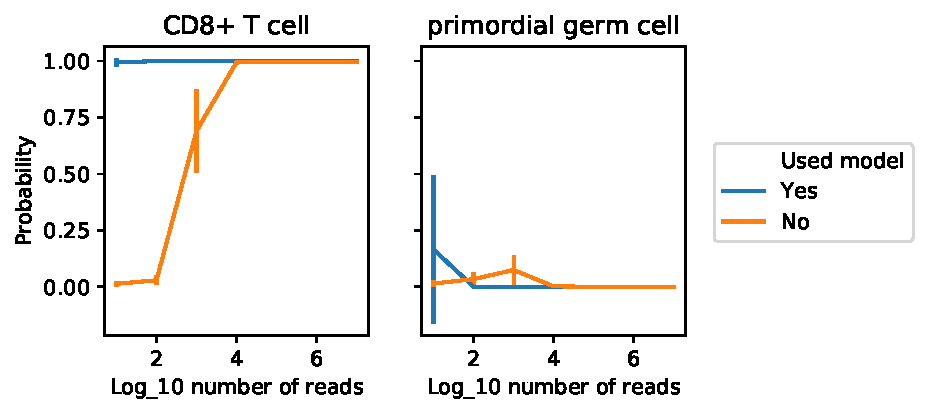
\includegraphics[width=13cm]{figures/downsample_apply_sc_model.pdf}}
      \caption{\textbf{Illustration of advantage of probabilistic model.} Results from the toy two-cell experiment demonstrating the potential advantages of this model. At each read-depth, 10 samples were generated from the CD8+ T cell sample (left) and the primordial germ cell sample (right).  At each read-depth, we plot the mean probability output by the default lymphocyte classifier (orange) and the mean probability output by the generative model-based lymphocyte classifier (blue) across the 10 samples. Error bars denote plus and minus one standard deviation around the mean.}
      \label{fig:sc_model_toy_experiment}
      \end{figure}
      
 \subsubsection{Performance on sparsified bulk RNA-seq test data}
 
 We evaluated this model by training it on the bulk RNA-seq training set and applying it to the sparsified versions of the bulk RNA-seq test set.  We explored a number of approaches for specifying the gamma-mixture distribution over the latent random variable $\bold{z}$, which entailed a number of clustering algorithms algorithms and methods for estimating the gamma parameters in each mixture component.  Specifically, we tested three clustering algorithms: agglomerative clustering with Pearson correlation distance using 500 clusters, using each cell type in the training set to define clusters, and finally, clustering the data \textit{within} each cell type and using the union of all clusters within all cell types.  We also tested two methods for estimating the parameters of each gamma distribution from the samples within each corresponding cluster: In the first variant, we use method of moments. In the second variant, we fit the mean using method of moments, but then perform an empirical Bayes-like approach to increase the variance when variance is low (thereby "smoothing" the gamma distributions).  We found that these various methods for estimating the gamma distributions yielded qualitatively similar performance and report here the best performing variant: using each cell type in the training data to define a cluster and performing the empirical Bayes-like procedure (Appendix~\ref{app:model_deriv}). 
 
In the per-cell type mode of evaluation, we found that this model tended to underperform the default classifiers at most read-depths, except the lowest (100 reads per sample).  Examining the performance across cell types, we found that the model severely underperformed in certain sections of the ontology.  For example, the model tended to perform poorly on epithelial cells, but comparably on lymphocytes (Fig.~\ref{fig:diff_cell_types}).  It is likely that this is due to the fact that the gamma distributions for these cell types are poorly fit. Future work will require further diagnosing the model in order to improve performance on these underperforming cell types. Because of the lower performance on many cell types, we decided to forego testing this model on the 10x dataset until future work could be carried out that would improve performance on these underperforming cell types.  By decreasing the number of times we evaluate this model on the 10x dataset, we mitigate the likelihood that modifications to the algorithm in response to the results will lead to overfitting on this dataset.

Nonetheless, when examining the performance in the per-sample and joint-modes of evaluation we find that this model produces better results than the default classifiers on all read-depths except the highest ($10^5$ reads per sample), which indicates two things. First, on common cell types, the model performs well, and second, the output probabilities of this model are much better calibrated across cell types than the default classifier's.  These results support our hypothesis that by imputing the genes, the input data better matches the data on which the models were trained and therefore calibrated.  Thus, this model offers a promising approach to scRNA-seq cell type classification, especially at extremely low read-depths. 

  \begin{figure}[htbp]
\centering
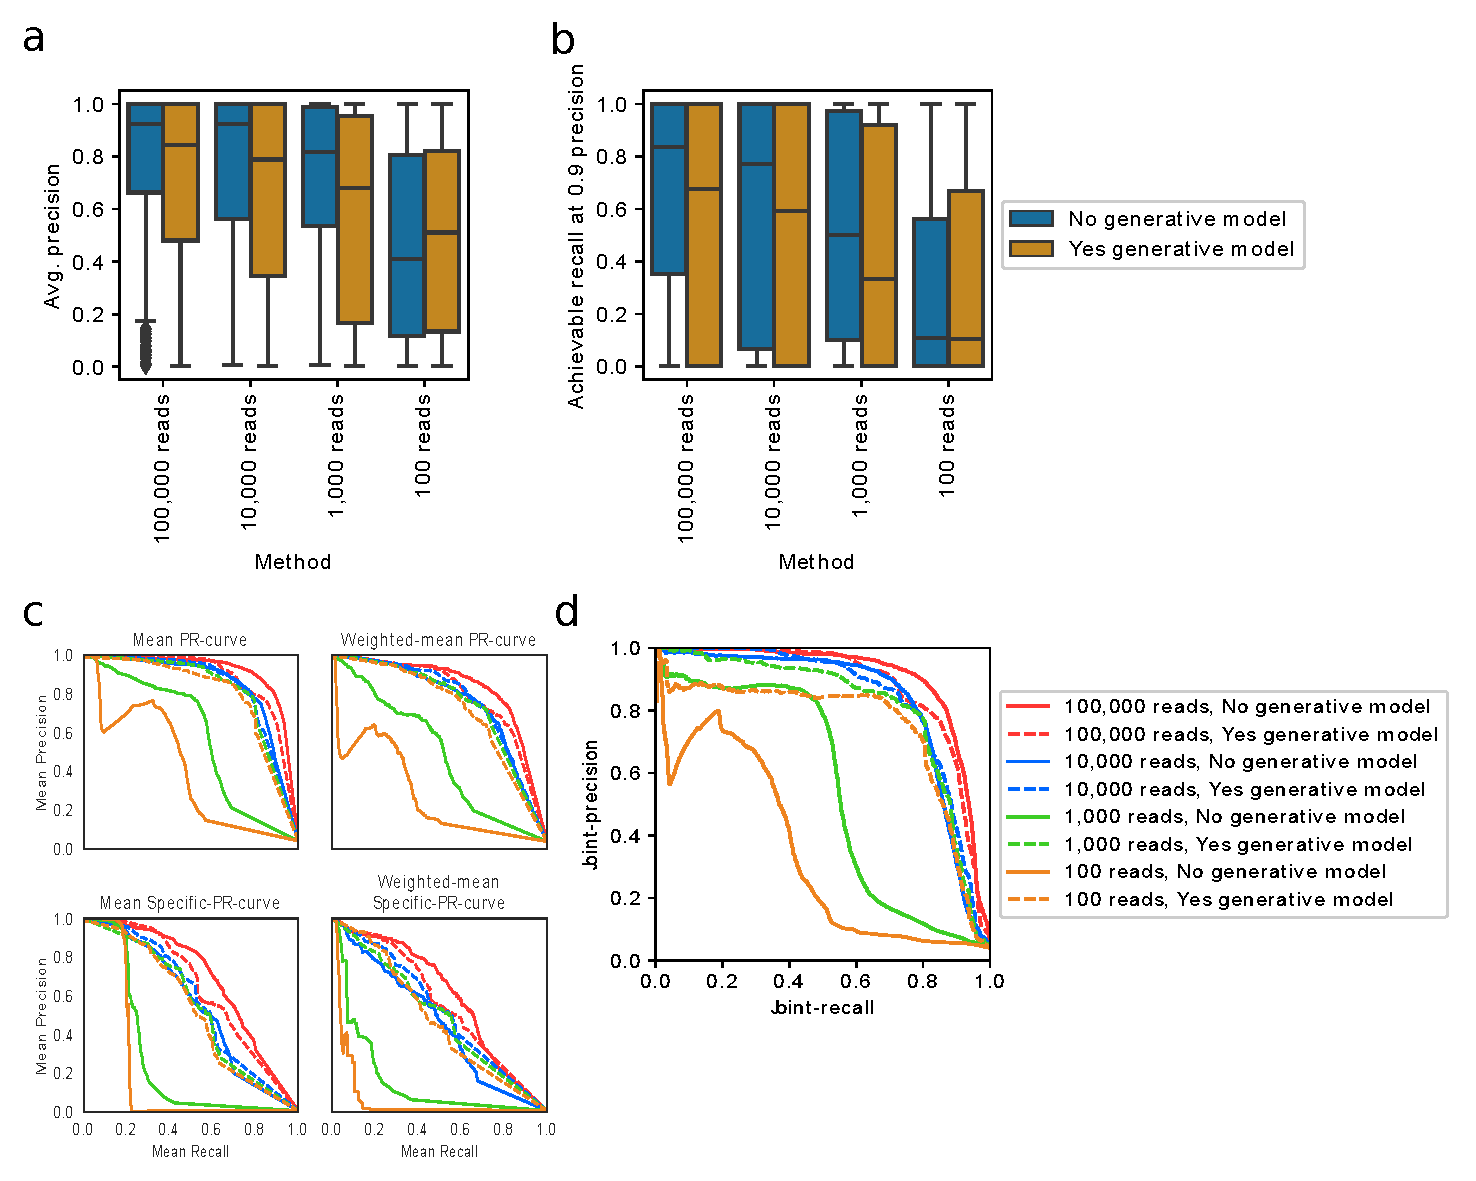
\includegraphics[width=13cm]{figures/new_model_results.pdf}  
\caption{\textbf{Results of the new model on the downsampled bulk RNA-seq test set.} (a) Comparison between the distributions of average-precision generated by each method across all cell types.  (b) Comparison of the distributions over the highest achievable recalls when precision is fixed at 0.9 across all cell types. (c) Variants of the mean precision-recall curves for comparing the average performance of each method across all samples. (d) The joint-precision recall curves for all methods generated by ranking all sample-cell type output probabilities jointly.}
\label{fig:diff_cell_types}
\end{figure}
 
 \begin{figure}[htbp]
\centering
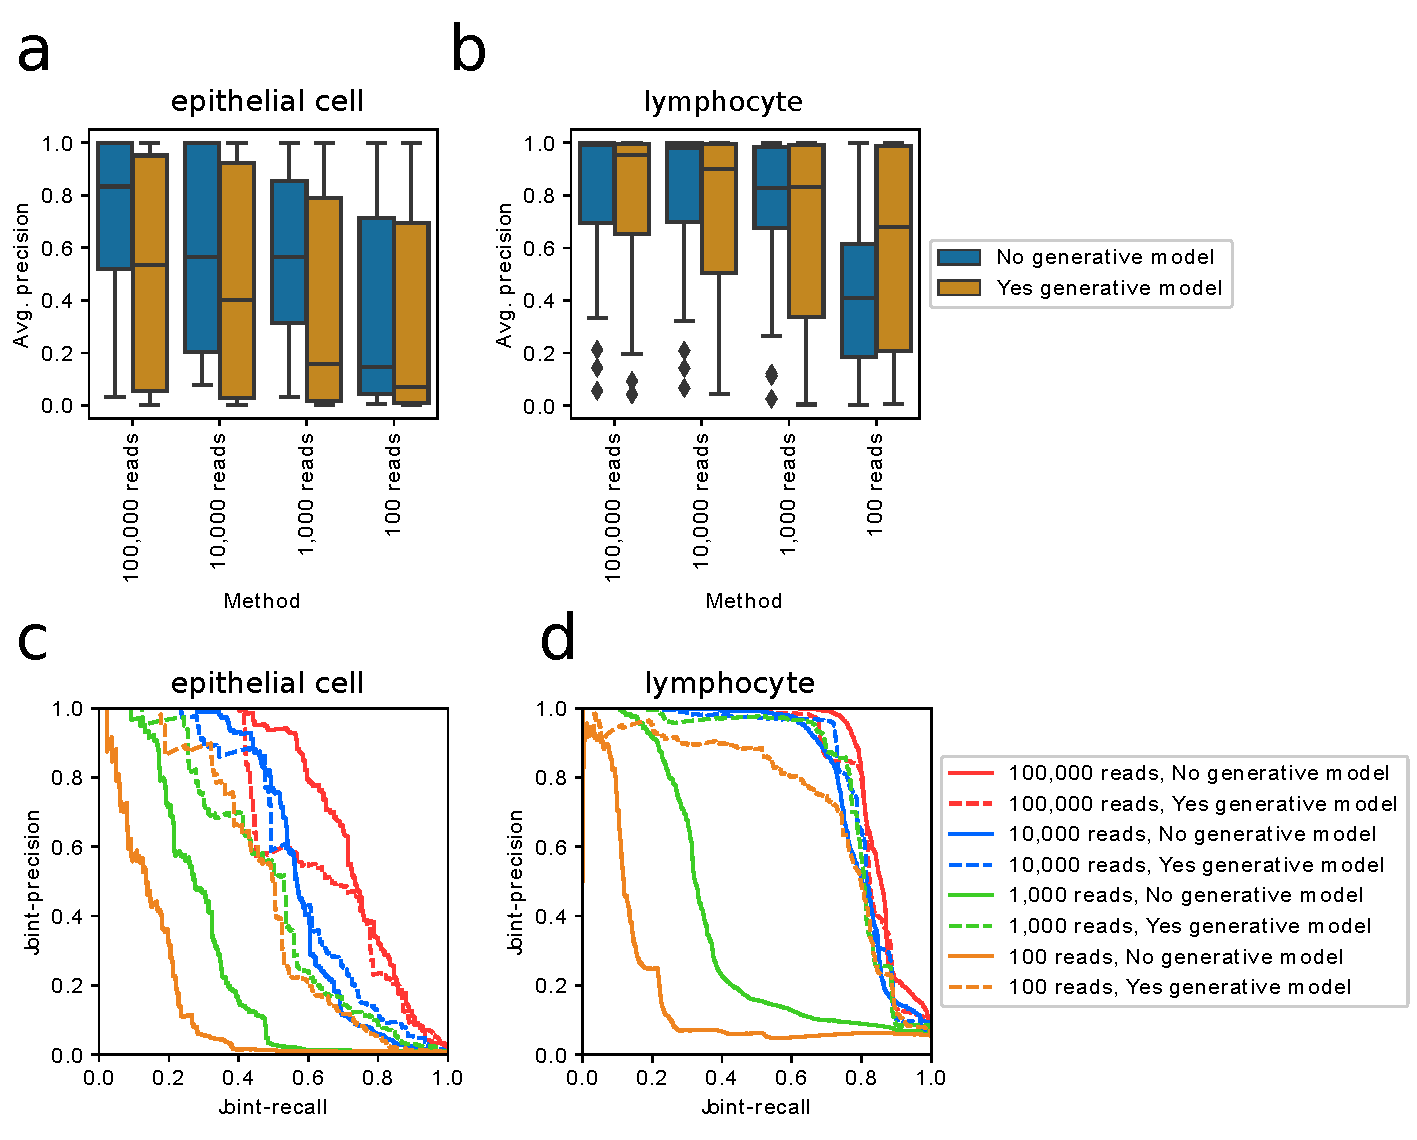
\includegraphics[width=13cm]{figures/paired_avg_precision_two_cell_types}  
\caption{\textbf{Performance of new model on differing sections of the ontology.} Comparing the distribution of average precision scores across cell types between the standard classifiers and the classifiers adapted with the probabilistic model. We compare the distributions across (a) epithelial cell types and (b) lymphocyte cell types. We also compare the join-precision-recall curves for (c) epithelial cell types and (d) lymphocyte cell types.}
\label{fig:diff_cell_types}
\end{figure}
 
%\subsubsection{Diagnosing the model}
      
\subsection{Conclusions and future work}

In this work, we explored approaches for extending the one-vs.-rest cell type classifiers developed in Chapter~\ref{chap:2} to sparse scRNA-seq data. Because these classifiers were trained on bulk RNA-seq data, they performed poorly on sparse data out of the box.  To address these shortcomings we explored methods for imputing the values for the genes in order for the test data to better resemble the dense training data.

To address these shortcomings, we explored two main approaches for adapting the classifiers developed in Chapter~\ref{chap:2}:
\begin{enumerate}
\item Training on artificially sparse bulk RNA-seq data in order for the training data to better resemble the sparse test data.
\item Imputing the values for the genes in order for the test data to better resemble the dense training data.
\end{enumerate}
When possible, we evaluated each strategy on both an artificially sparse bulk RNA-seq test set as well as a dataset of droplet-based 10x scRNA-seq expression profiles consisting of various peripheral blood mononuclear cell types. 

Unsurprisingly, we found that training on artificially sparse bulk RNA-seq data led to better performance than the default, out-of-the-box classifiers.  However, this gain in performance requires training a classifier at a read-depth that matches the test set. Since our goal is to train a single classifier for use on scRNA-seq datasets of varying read-depths, we explored the use of gene expression imputation algorithms that would enable training the classifier only once. We found that imputing the values of the genes with MAGIC led to improved performance.  This indicates that pre-processing the query data with a gene expression imputation algorithm will improve the results of cell type classifiers trained on bulk RNA-seq data.  Future work will involve benchmarking other recent imputation algorithms, such as SAVER, for the cell type classification task. 

 Lastly, because gene expression imputation requires expensive computation at test-time, we explored a novel method for classification of sparse scRNA-seq data based on a generative model of the scRNA-seq data-generating process. This model outperformed the default classifiers on the per-sample and joint-modes of evaluation.  Most promisingly, at very low read-depths, this model provided results that were competitive with those from higher read-depths. Nonetheless, we found that the model suffered on certain cell types. Future work will require diagnosing the cause for the poorer performance on these cell types. Nonetheless, these results reveal a promising direction towards the goal of developing a robust, well-calibrated classifier for classifying sparse scRNA-seq data against the full breadth of the Cell Ontology.  


 





